% !TEX root = ../main.tex

\section{Background}
\subsection{How attack could happen}
The attack can occur in case of race condition\footnote{Execution of two transactions at the same time with undesirable situation.}. It allows spender to transfer more tokens than the owner ever wanted. This is possible by executing \textit{transferFrom} function two times, before and after the \textit{approve} method. According to ERC20 API definition:
\begin{enumerate}[label=(\alph*)]
	\item \textit{approve}\footnote{approve(address \textit{\_spender}, uint256 \textit{\_tokens})} function allows \textit{\_spender} to withdraw up to the \textit{\_value} amount of tokens from token pool of the approver. If this function is called again, it has to overwrites the current allowance with the new \textit{\_value}.
	\item \textit{transferFrom}\footnote{transferFrom(address \textit{\_from}, address \textit{\_to}, uint256 \textit{\_tokens})} function grants required rights to the spender (account, wallet or other smart contract) for transferring \textit{\_value} amount of tokens from address \textit{\_from} to address \textit{\_to}.
\end{enumerate}
Attacker can take advantage of the gap between execution of \textit{approve} and \textit{transferFrom} functions since the \textit{approve} method overrides current allowance regardless of whether spender already transferred any tokens or not. Transferred tokens are not trackable and only \textit{Transfer}\footnote{Transfer(address indexed \textit{\_from}, address indexed \textit{\_to}, uint256 \textit{\_value})} event will be logged which is not sufficient in case of transferring tokens to a third parity. To make it more clear, the following attack scenario can be considered:
\begin{enumerate}
	\item Alice allows Bob to transfer N tokens on her behalf by calling \textit{approve(\_Bob, N)}.
	\item After a while, Alice decides to change Bob's approval from N to M by executing \textit{approve(\_Bob, M)}.
	\item Bob notices Alice’s second transaction before it was mined and quickly sends another transaction that runs \textit{transferFrom(\_Alice, \_Bob, N)}. This will transfer N Alice’s tokens to Bob.
	\item Bob’s transaction will be executed before Alice’s transaction (because of higher transaction fee, miner’s policy or other prioritization techniques) and Bob front-runs Alice’s transaction.
	\item Alice’s transaction will be executed after Bob’s and allows Bob to transfer more M tokens.
	\item Bob successfully transferred N Alice’s tokens before and gains ability of transferring another M tokens.
	\item Before Alice notices that something went wrong, Bob calls \textit{transferFrom} method for the second time and transfers M Alice’s tokens by executing \textit{transferFrom(\_Alice, \_Bob, M)}.
\end{enumerate}
In fact, Alice attempted to change Bob’s allowance from N to M, but she made it possible for Bob to transfer N+M of her tokens at most, while Alice never wanted to allow so many transfers to be occurred by Bob. It should be noted that the assumption here is to prevent Bob from withdrawing Alice’s tokens multiple times when allowance changes from N to M. If Bob could withdraw N tokens after Alice initial approval, this would be considered as legitimate transfer, since Alice has already approved it. In other words, it would be responsibility of Alice to make sure before approving anything to Bob. After approval, Bob is allowed to transfer up to N tokens even right before allowance change. In the below figure, transaction \#4 would be considered as multiple withdrawal attack since Bob is able to move more M tokens in addition to already transferred N tokens in step \#3.
\begin{figure}[h]
	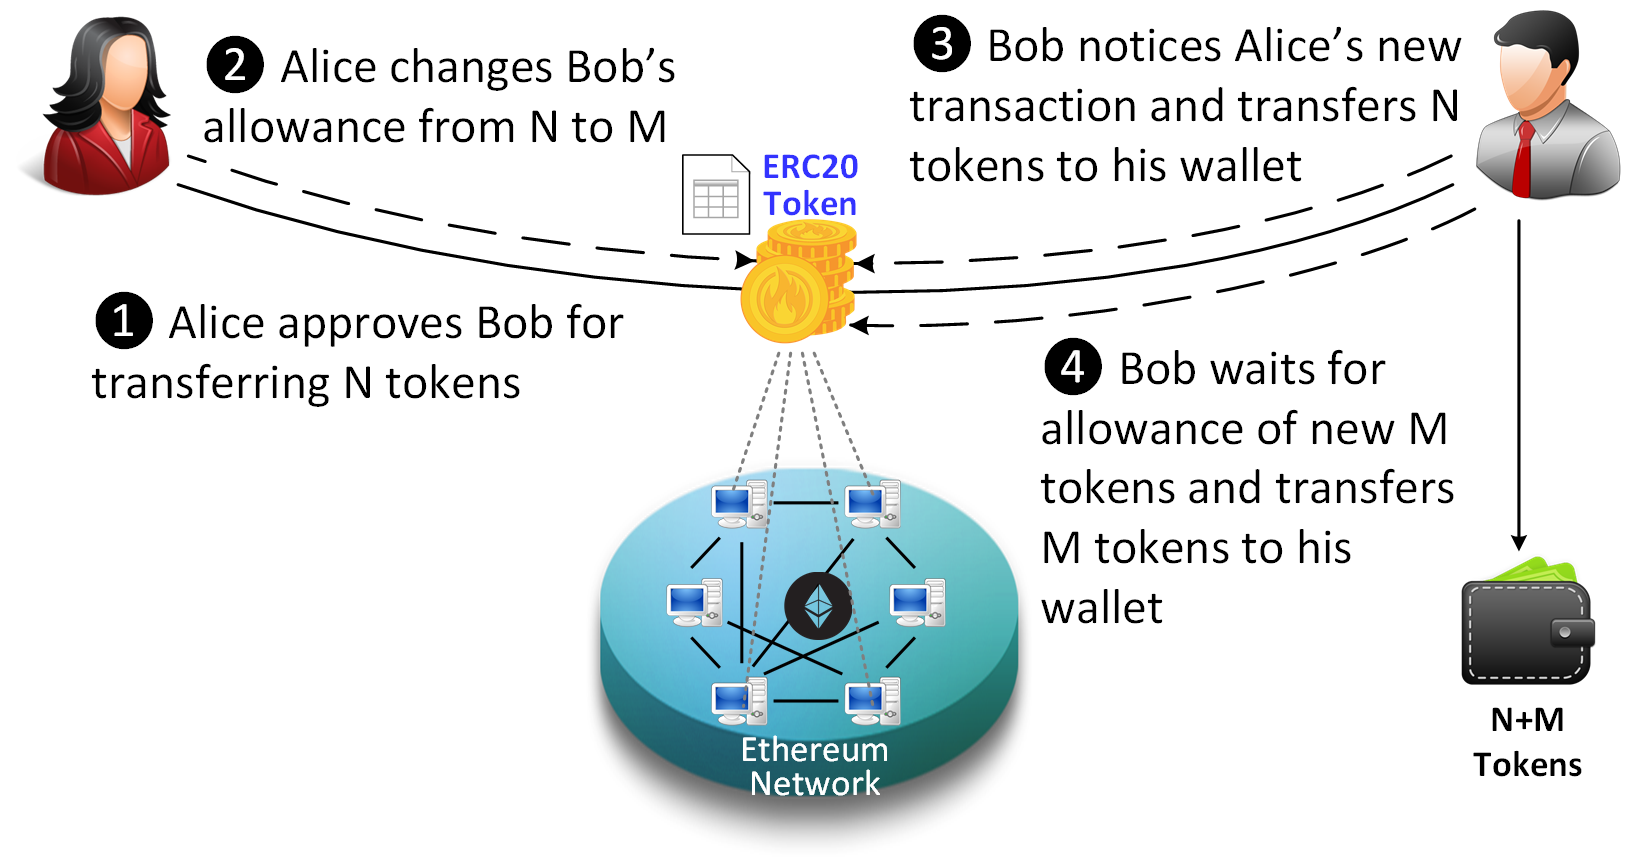
\includegraphics[width=1.0\linewidth]{figures/multiple_withdrawal_02.png}
	\caption{Possible multiple withdrawal attack in ERC20 tokens when Alice changes Bob's allowance from N to M. By front-running, Bob is able to move N+M tokens from Alice's token pool.}
\end{figure}

\subsection{How to prevent the attack}
A sustainable solution has to prevent the attack by securing \textit{approve} or \textit{transferFrom} functions. As a third approach, ERC20 standard left it to owner:\newline

\begin{enumerate}[label=\Roman*.]
	\item \textbf{Prevention by owner:} This approach is recommended by ERC20 standard \cite{Ref08} and advises owners to change spender allowance from N to 0 and then from 0 to M (instead of set it directly from N to M). Changing allowance to non-zero values after setting to zero will not prevent the attack since the owner would not be able to distinguish how the allowance was set to zero. Was it because of previous \textit{approve} transaction for changing allowance from N to 0?, Or it was set to 0 by \textit{transferFrom} method due to token transfers? Although It would be possible to track transferred token through \textit{Transfer} events, tracking of tokens would not be easy in case of transferring to a third-party. For example, if Alice allows Bob and then Bob transfers tokens to Carole, \textit{Transfer} event creates a log showing Carole moved tokens from Alice. As discussed in "MiniMeToken", this approach can not prevent the attack since it is not distinguishable which transaction (i.e., owner or attacker transaction) has set allowance to zero.\newline
	
	\item \textbf{Prevention by \textit{approve} method:} By using compare and set (CAS) pattern \cite{Ref06} in this approach, \textit{approve} method can change spender allowance from N to M atomically. Comparison part of CAS requires knowledge of transferred tokens that reveals any transferred tokens in case of front-running. Hence, we can compare new allowance with transferred token and set it accordingly. Although this is promising approach, but setting new allowance in \textit{approve} method must satisfy ERC20 constraint that says "If this function is called again it overwrites the current allowance with \textit{\_value}" \cite{Ref08}. In other words, any adjustments in allowance is prohibited which makes the \textit{approve} method vulnerable. For example, considering front-running by Bob when Alice wants to change Bob allowance form 100 to 110, the \textit{approve} method can reveal 100 transferred tokens by Bob. However, based on ERC20 constraints, it must not adjust new allowance to 110-100=10, it has to set it literally to 110, which is allowing Bob for transferring 100+110=210 tokens in total. We implemented this approach in proposal 1 and conlcuded that securing \textit{approve} method can not prevent the attack while adhering constraints of the ERC20 standard.\newline
	
	\item \textbf{Prevention by \textit{transferFrom} method:} Based on ERC20 constraint, "approve functions allows \textit{\_spender} to withdraw from your account multiple times, up to the \textit{\_value}". Hence, spender must not be able to transfer more than authorized tokens. That being said, \textit{transferFrom} method can be secured in a way that prevents M new tokens transfer in case of already transferred N tokens. By comparing transferred tokens in \textit{transferFrom} method, spender will be restricted to move solely remained tokens of his allowance. In case of trying to transfer more tokens than allowed, the transaction fails. For example, Alice's new transaction for increasing Bob allowance from 100 to 110, sets Bob allowance to 110 (since the \textit{approve} method does not adjust allowance). However, \textit{transferFrom} method does not allow Bob from transferring more than 10 tokens if he had already transferred 100 tokens. We implemented this approach in proposal 2 and it prevents the attack effectively.
\end{enumerate}

\subsection{What are properties of acceptable solutions}
An important criterion for a solution is to adhere the specifications of ERC20 standard. Conforming with the standard, keeps new tokens backward compatible with already deployed smart contracts. So, smart contracts can interact with tokens as defined in the standard without raising any runtime exception. We summarized defined constraints from ERC20 specifications \cite{Ref08} that must be satisfied by any sustainable solution:
\begin{enumerate}
	\item Calling \textit{approve} function has to overwrite current allowance with new allowance.
	\item \textit{approve} method does not adjust allowance, it sets new value of allowance.
	\item Transferring 0 values by \textit{transferFrom} method MUST be treated as normal transfers and fire the \textit{Transfer} event as non-zero transactions.
	\item Introducing new methods violates ERC20 API and it MUST be avoided for having compatible token with already deployed smart contracts.
	\item Spender will be allowed to withdraw from approver account multiple times, up to the allowed amount.
	\item Transferring initial allowed tokens is considered as legitimate transfer. It could happen right after approval or before changing allowance.
	\item Race condition MUST not happen in any case to prevent multiple withdrawal from the account.\newline
\end{enumerate}